\subsection{Reluktanz-Schrittmotor}
\begin{minipage}{0.5 \linewidth}
\subsubsection{Wirkungsprinzip}
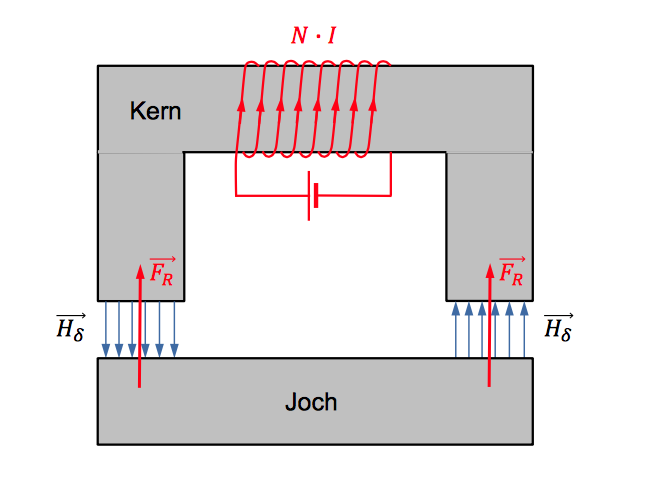
\includegraphics[width = \linewidth]{./Pics/VL67/WirkungRe}
Die magnetische Reluktanzkraft ist immer anziehen, d.h. die Reluktanzkraft versucht die Luftspalte zu verkleinern oder völlig zu eliminieren.
\end{minipage}
\begin{minipage}{0.5 \linewidth}
\subsubsection{Aufbau}
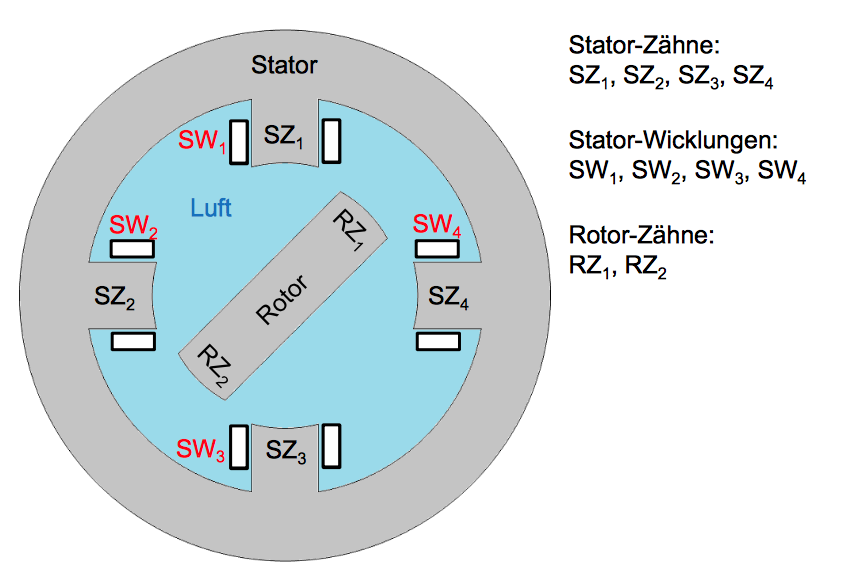
\includegraphics[width = \linewidth]{./Pics/VL67/AufbauRe}
\end{minipage}

\begin{minipage}{0.5 \linewidth}
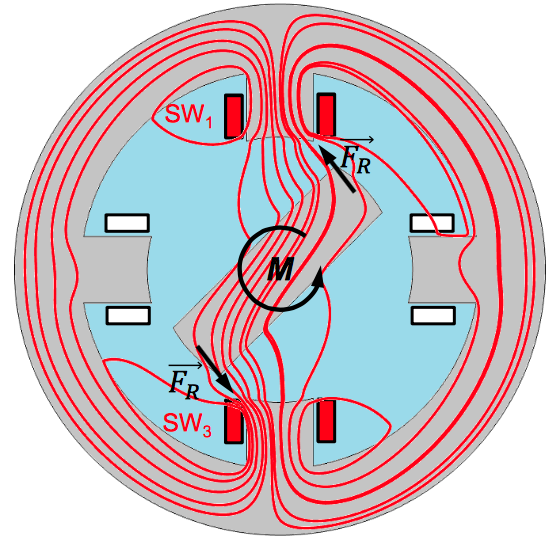
\includegraphics[width = 0.7 \linewidth]{./Pics/VL67/WirkungRe2}
\end{minipage}
\begin{minipage}{0.5 \linewidth}
\begin{itemize}
\item Die Spulen $SW_1$, $SW_3$ sind an die Quelle angeschlossen.
\item Das magnetische Feld der ersten zwei Spulen wird erzeugt.
\item Die Reluktanzkraft wirkt auf den Rotor um die Luftspalte zu verringern.
\item Das mechanische Moment wird erzeugt. 
\end{itemize}
\end{minipage}

\subsection{Permanentmagnet-SM}
\begin{minipage}{0.5 \linewidth}
\subsubsection{Wirkungsprinzip}
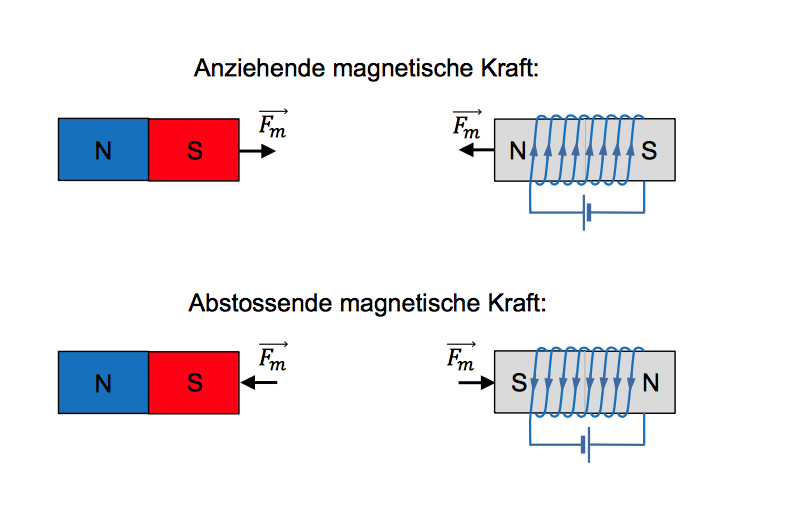
\includegraphics[width = \linewidth]{./Pics/VL67/PMSM2}
\end{minipage}
\begin{minipage}{0.5 \linewidth}
\subsubsection{Aufbau}
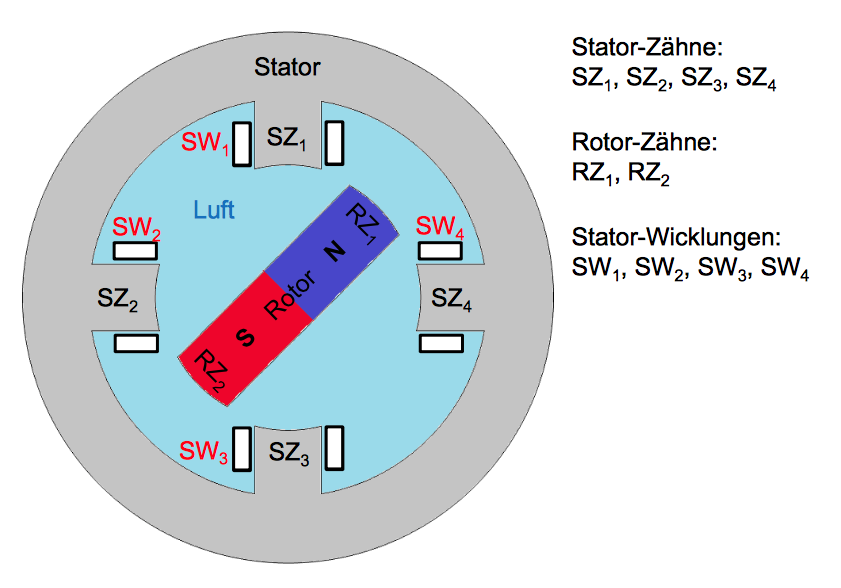
\includegraphics[width = \linewidth]{./Pics/VL67/PMSM}
\end{minipage}

\subsection{Grundgleichungen}
\begin{minipage}{0.5 \linewidth}
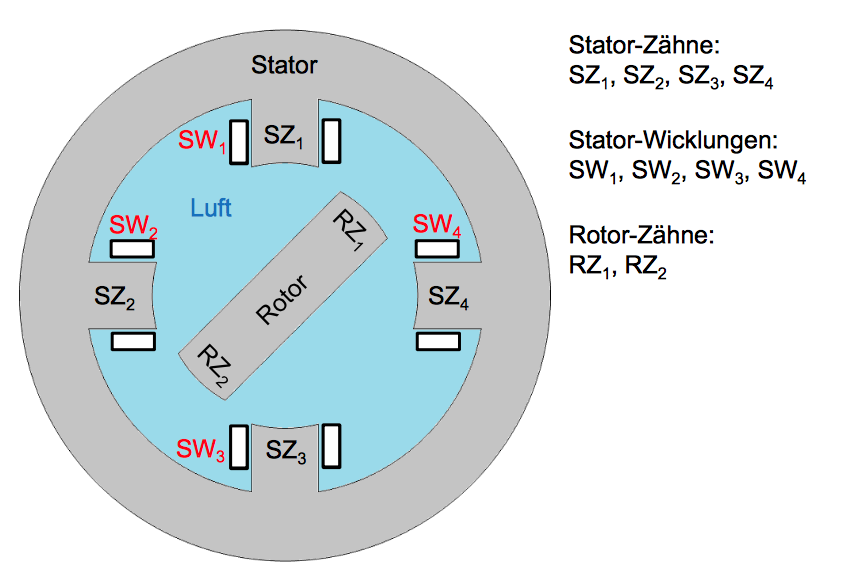
\includegraphics[width = \linewidth]{./Pics/VL67/AufbauRe}
\end{minipage}
\begin{minipage}{0.5 \linewidth}
\subsubsection{Aufbau}
\begin{compactitem}
\item Die Stator-Spulen sind an die Quelle der Steuersignale angeschlossen.
\item Die Steuersignale produzieren das schrittweise Drehen der Motorwelle.
\item Die Stator-Zahnzahl: $Z_S = 4$
\item Die Rotor-Zahnzahl: $Z_R = 2$
\item Der Stator-Winkel: $\alpha_S = \frac{2\cdot \pi}{Z_S} = 90^\circ$
\item Der Rotor-Winkel: $\alpha_R =  \frac{2\cdot \pi}{Z_R} = 180^\circ$
\item Der Vollschritt-Winkel: $\alpha_0 = \alpha_R - \alpha_s = 90^\circ$ 
\item Der Vollschritt-Winkel bezeichnet die Bewegung des Rotors pro Einzelsteuerimpuls.
\item Die Strangzahl: $m = \frac{Z_S}{Z_S - Z_R} = 2$
\item Die Schrittzahl: $N_p = \frac{2\cdot \pi}{\alpha_0} = 4$
\item Die Steuerfrequenz: $f_s = N_p \cdot \frac{n}{60}$ 
\item Das Drehmoment: $M_M = \frac{1}{2} \frac{L_d-L_q}{a_0} \cdot I^2_1$
\end{compactitem}
\end{minipage}

\subsection{Drehmoment}
\begin{minipage}{0.5 \linewidth}
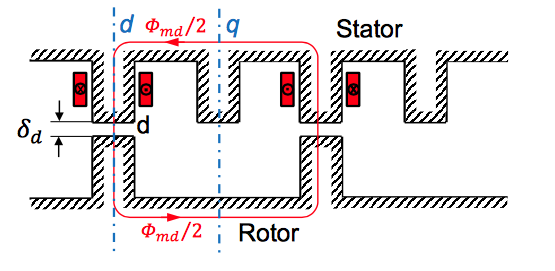
\includegraphics[width = 0.9\linewidth]{./Pics/VL67/Drehmoment}\\
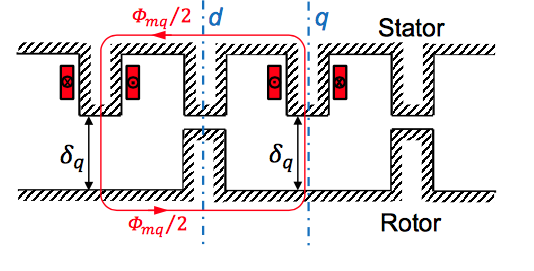
\includegraphics[width = 0.9\linewidth]{./Pics/VL67/Drehmoment2} \\

Der magnetische Fluss des Motors: \\

$\Phi_m (\gamma_r,i) = L(\gamma_r(t)) \cdot i(t)$\\

Die Spannung des Statorkreises: 

$u(t)  = R \cdot i(t) + \frac{d\Phi_m}{dt}(t)  = R \cdot i(t) + \frac{d}{dt}(L(\gamma_r(t) \cdot i(t)) \\
 =  R \cdot i(t) + \frac{dL}{d\gamma_r}(\gamma_r) \cdot \frac{d\gamma_r}{dt}i(t) + L(\gamma_r) \cdot \frac{di}{dt}(t)$ \\
 
 Die Leistung des Statorkreises: \\
 
 $p(t) = u(t) \cdot i(t) = R \cdot i^2(t) + \frac{dL}{d\gamma_r} \cdot \omega_r \cdot i^2(t) + L \cdot i(t) \cdot \frac{di}{dt}(t)$\\
 
 Die elektrische Leistung des Stators: 
 
 $p(t) = R \cdot i^2(t) + \frac{dL}{d\gamma_r} \omega_r \cdot i^2(t) + L \cdot i(t) \cdot \frac{di}{dt}(t) \\ 
 = p_{C_u}(t) + \frac{d_{W_m}}{dt}(t) + \frac{1}{2} \cdot \frac{dL}{d \gamma_r}(\gamma_r) \cdot \omega_r \cdot i^2(t)$ \\
 
\end{minipage}
\begin{minipage}{0.5 \linewidth}
Die Induktivität des Statorstrangs (Die Position der d-Achse des Rotor parallel mit dem aktivem Statorzahn): \\

$L_d = 2 \cdot N \frac{\Phi_{md}}{I_1} = 2 \cdot N \frac{B_{\delta d} \cdot A_z}{I_1} = \mu_0 \cdot 2 \cdot N \frac{2 \cdot N \cdot I_1 \cdot A_z}{2 \cdot \delta_d \cdot I_1} = \mu_0 \cdot 2 \cdot N^2 \frac{A_Z}{\delta_d}$ \\

wobei $N$ die Windungszahl des Statorstrangs, $A_Z$ die Zahnfläche und $\delta_d$ die Höhe des Luftspalts (bei der d-Position des Rotors relativ zu dem Statorzahn) ist. \\
Die Induktivität des Statorstrangs hängt offenbar von der Rotorposition ab: \\

$L_q = \frac{\Psi_{m2}}{I_1} = 2N \frac{\Phi_{m2}}{I_1} = 2 \cdot N \frac{B_{\delta2 \cdot L \cdot w_{zu}}}{I_1} = 2 \cdot N \cdot \mu_0 \frac{2 \cdot N \cdot I_1} \cdot L \cdot w_{zu}{2\delta \cdot I_1} = 2 \cdot \mu_0 N^2 \frac{L\cdot w_zu}{\delta}$ \\

Wobei $w_{zu}$ die Breite der Zahnüberlappung in der q-Position ist: \\

$w_{zu} = w_s - a_0 \cdot \frac{D \cdot \pi}{360^\circ} $ \\

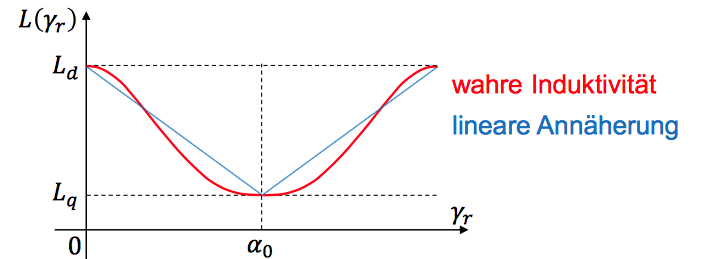
\includegraphics[width = 0.8 \linewidth]{./Pics/VL67/Drehmoment3} \\
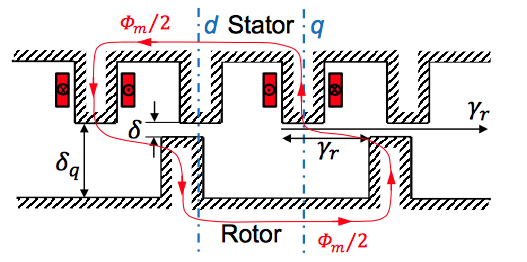
\includegraphics[width = 0.9 \linewidth]{./Pics/VL67/Drehmoment4} \\
\end{minipage}

\begin{minipage}{0.5 \linewidth}
Die Zeitableitung der magnetischen Energie: \\

$w_m(t) = \frac{1}{2} L(\gamma_r) \cdot i^2(t) \Rightarrow \frac{d}{dt}(\frac{1}{2}\cdot L(\gamma_r)\cdot i^2(t)) = \\
\frac{1}{2} \cdot \frac{dL}{d\gamma_r}(\gamma_r) \cdot \omega_r \cdot i^2(t) + L \cdot i(t) \cdot \frac{di}{dt}(t)$ \\

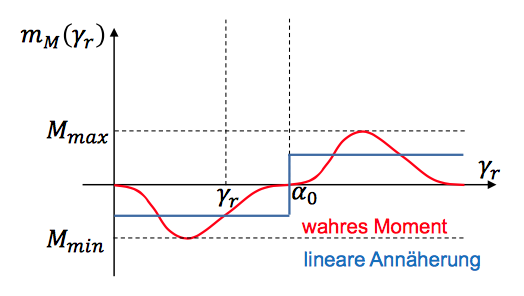
\includegraphics[width = \linewidth]{./Pics/VL67/Drehmoment5}
\end{minipage}
\begin{minipage}{0.5 \linewidth}
Die Rotorleistung: \\

$P_\delta (t) = \frac{1}{2} \cdot \frac{dL}{d\gamma_r}\cdot(\gamma_R) \cdot \omega_r \cdot i^2(t)$ \\

Das Motormoment: 

$m_M(t) = \frac{p_\gamma}{\omega_r}(t) = \frac{1}{2} \cdot \frac{dL}{d\gamma_r}(\gamma_r) \cdot i^2(t)$\\

Das Betriebsverhalten des Motors beschreibt die folgende Gleichung: 

$J_g \frac{d\omega_r}{dt} = M_M - M_L $\\

wobei $J_g$ das gesamte motorbezogene Trägheitsmoment des System, $M_M$ das Drehmoment des Motors und $M_L$ das Widerstandsmoment der Last ist.\\
\end{minipage}

\begin{minipage}{0.5 \linewidth}
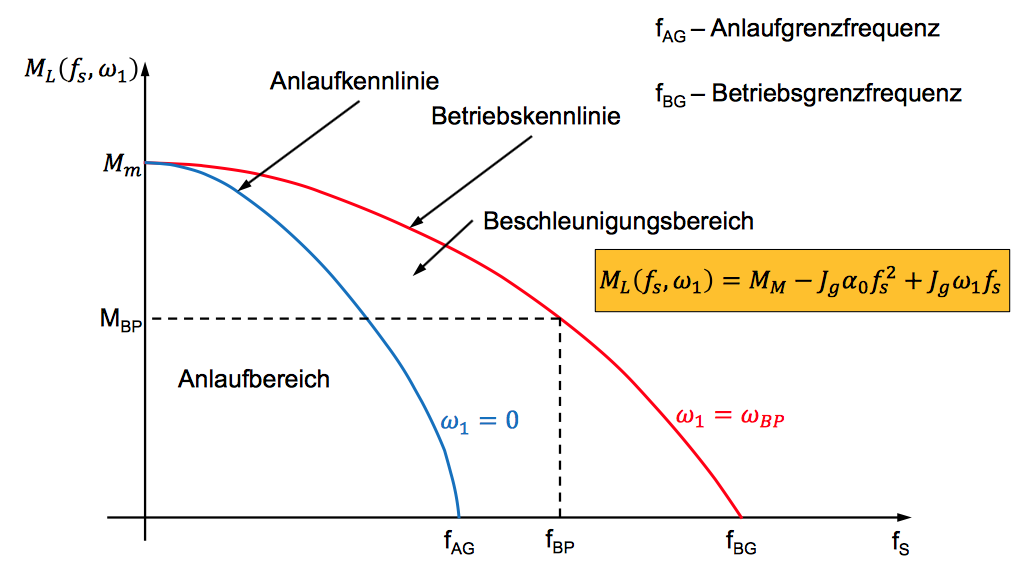
\includegraphics[width = \linewidth]{./Pics/VL67/Betriebsverhalten}
\end{minipage}
\begin{minipage}{0.5 \linewidth}
Die Differenzialgleichung der Rotorbewegung (mit der linearen Annäherung der Winkelbeschleunigung): \\

$J_g \frac{\omega_s-\omega_1}{T_s} = M_M - M_L$ \\

wobei $\omega_s = 2 \cdot \pi \frac{n_s}{60} = 2 \cdot \pi \frac{f_s}{N_p} = a_0 f_s$ die Kreisgeschwindigkeit des Statorfelds, $\omega_1$ die geometrische Kreisgeschwindigkeit des Rotors in dem Moment des Impulseinschaltens ($\omega_1 = 0$ bedeutet der Rotor im Stillstand), $f_s = \frac{1}{T_s}$ die Frequenz der Statorimpulse ist. \\

Die Gleichung beschreibt die Beschleunigung des Rotors während einem Statorimpuls. Der Rotor muss von der Geschwindigkeit $\omega_1$ auf die Geschwindigkeit $\omega_s$ beschleunigen. Sonst wird der Rotor ausser Tritt geraten. \\

Das Lastmoment $M_L$ als eine Funktion der Schaltfrequenz und Anfangsgeschwindigkeit: \\

$M_L(f_s,\omega_1) = M_M-J_g\frac{\omega_s}{T_s} + J_g\frac{\omega_1}{T_s} \\
= M_M-J_g\omega_s f_s + J_g \omega_1 f_s\\
= M_M - J_g \alpha_0 f_s^2 + J_g \omega_1 f_s$\\
\end{minipage}

\begin{minipage}{0.5 \linewidth}
\subsection{Anwendungsbereich und Schlussanmerkung}
\begin{itemize}
\item Die Schrittmotoren sind für die Anwendung mit Bewegungsführung geeignet.
\item Die Schrittmotoren sind sehr kostengünstig.
\item Die Schrittmotoren sind praktisch nicht überlastbar.
\item Die wichtigsten Anwendungen:
\begin{itemize}
\item Arbeitsmaschine
\item Datenausgabegeräte (Plotter, Drucker, usw.)
\end{itemize}
\item Die Schrittmotoren geben einen Drehmoment von bis zu 5 Nm ab.
\item Die Schrittmotoren werden im unteren Leistungsbereich eingesetzt. 
\end{itemize}
\end{minipage}
\begin{minipage}{0.5 \linewidth}
\subsection{Drehzahlregelung und Anlauf}
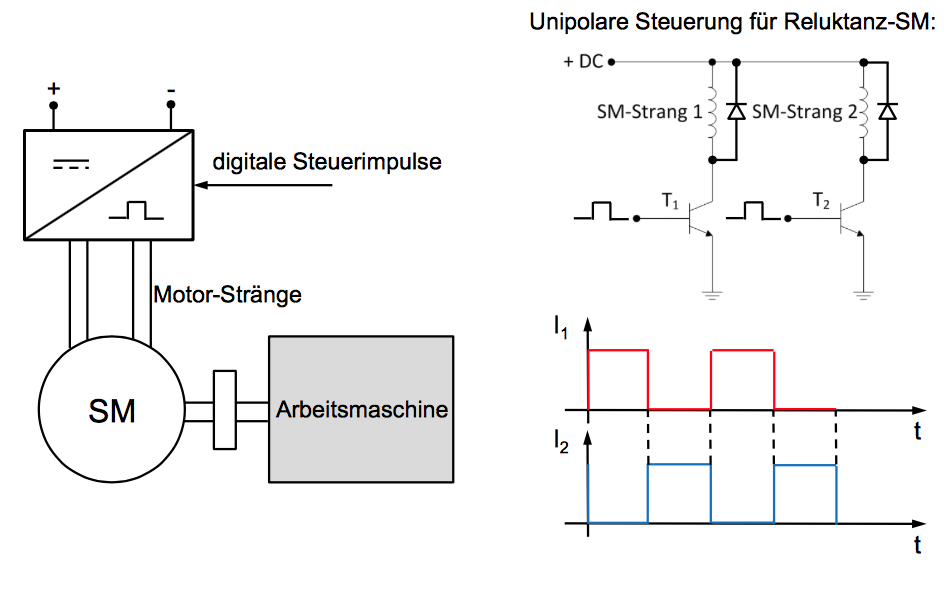
\includegraphics[width = \linewidth]{./Pics/VL67/Drehzahl}
\end{minipage}
